\subsection{Motivation}

\begin{frame}{Equilibrium climate sensitivity (ECS)}

    Simple energy balance model:
    \begin{equation}
        C\frac{\mathrm{d}\Delta T}{\mathrm{d}t}=-\frac{1}{s}\Delta T+f
    \end{equation}

    \vspace{-7mm}
    \visible<2>{
        \begin{equation*}
            \downarrow
        \end{equation*}
        \begin{equation}
            \Delta T=sf_{2\times\ce{CO2}}
        \end{equation}

    \(\Delta T\sim\) Equilibrium climate sensitivity (ECS)
    }

    \note<+>{
        \begin{itemize}
            \item Starting with very simple linear EBM
        \end{itemize}
    }
    \note<+>{
        \begin{itemize}
            \item (Equilibrium) Climate sensitivity is a measure of temperature
                change to a radiative imbalance
            \item Large \(\rightarrow\) strong response to forcing and large temperature change,
                small \(\rightarrow\) modest response and small temperature change
            \item Robust feature of sophisticated models for different forcings. To
                first order the magnitude of the forcing is what matter, not the
                type (e.g.\ infrared vs.\ shortwave)
            \item Gives a simple measure of the severity of global warming
        \end{itemize}
    }

\end{frame}

\begin{frame}{Estimating ECS}

    \begin{figure}
        \centering
        \begin{tikzpicture}
            \node[anchor=south west,inner sep=0] at (0,0) {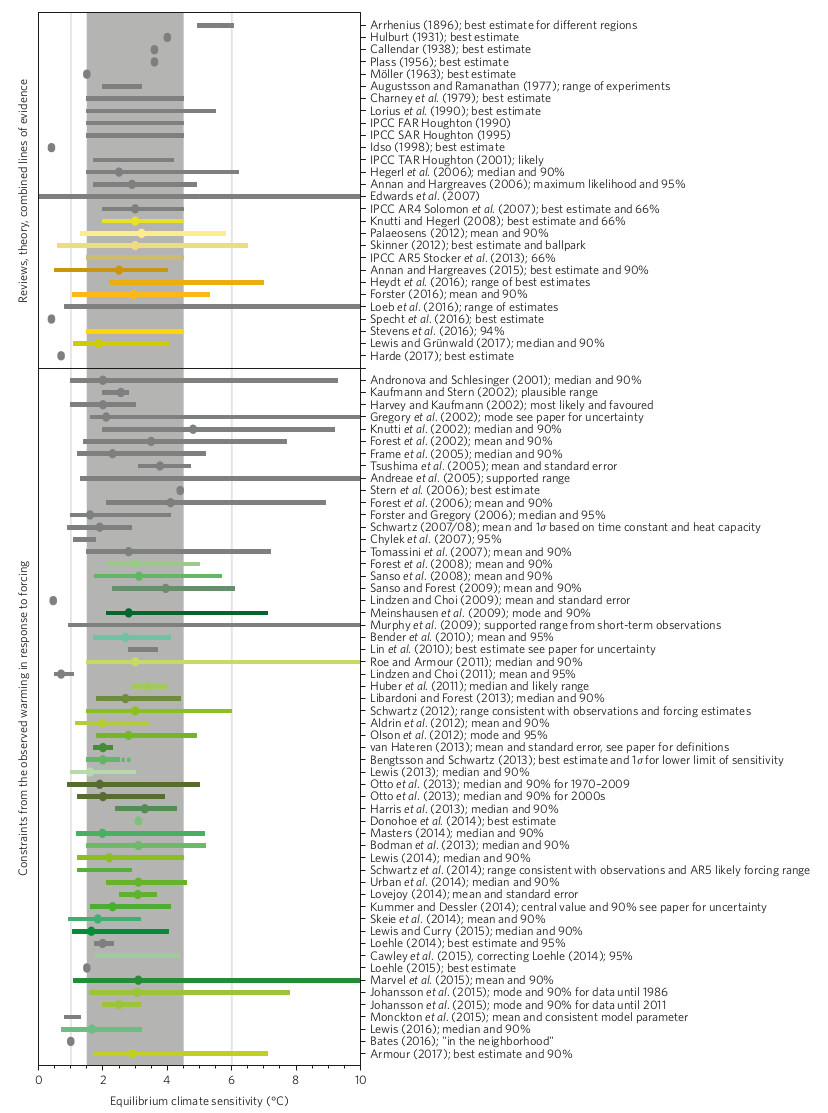
\includegraphics[width=.4\linewidth]{pic/equilibrium_climate_sensitivity.png}};
            \draw[white,anchor=south west,fill] (0.1,0.02) rectangle (1.6,0.1);
            \node[red,anchor=south west,inner sep=0] at (2.1,0.0) {\scalebox{.4}{ECS ($\mathrm{^\circ C}$)}};
            \node[red,anchor=south west,inner sep=0] at (0.16,0.02) {\scalebox{.4}{$0$}};
            \node[red,anchor=south west,inner sep=0] at (0.35,0.02) {\scalebox{.4}{$1.5$}};
            \node[red,anchor=south west,inner sep=0] at (0.85,0.02) {\scalebox{.4}{$4.5$}};
            \node[red,anchor=south west,inner sep=0] at (1.83,0.02) {\scalebox{.4}{$10$}};
        \end{tikzpicture}
        % 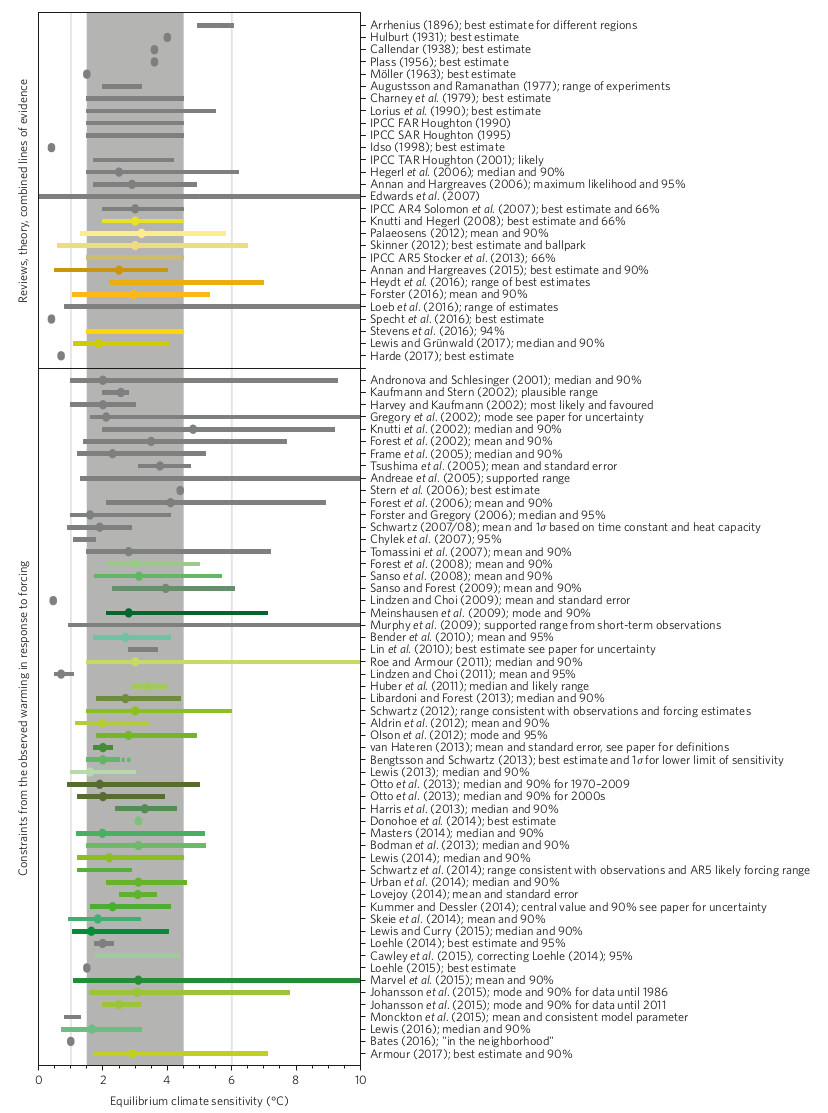
\includegraphics[width=.4\linewidth]{pic/equilibrium_climate_sensitivity.png}
        % 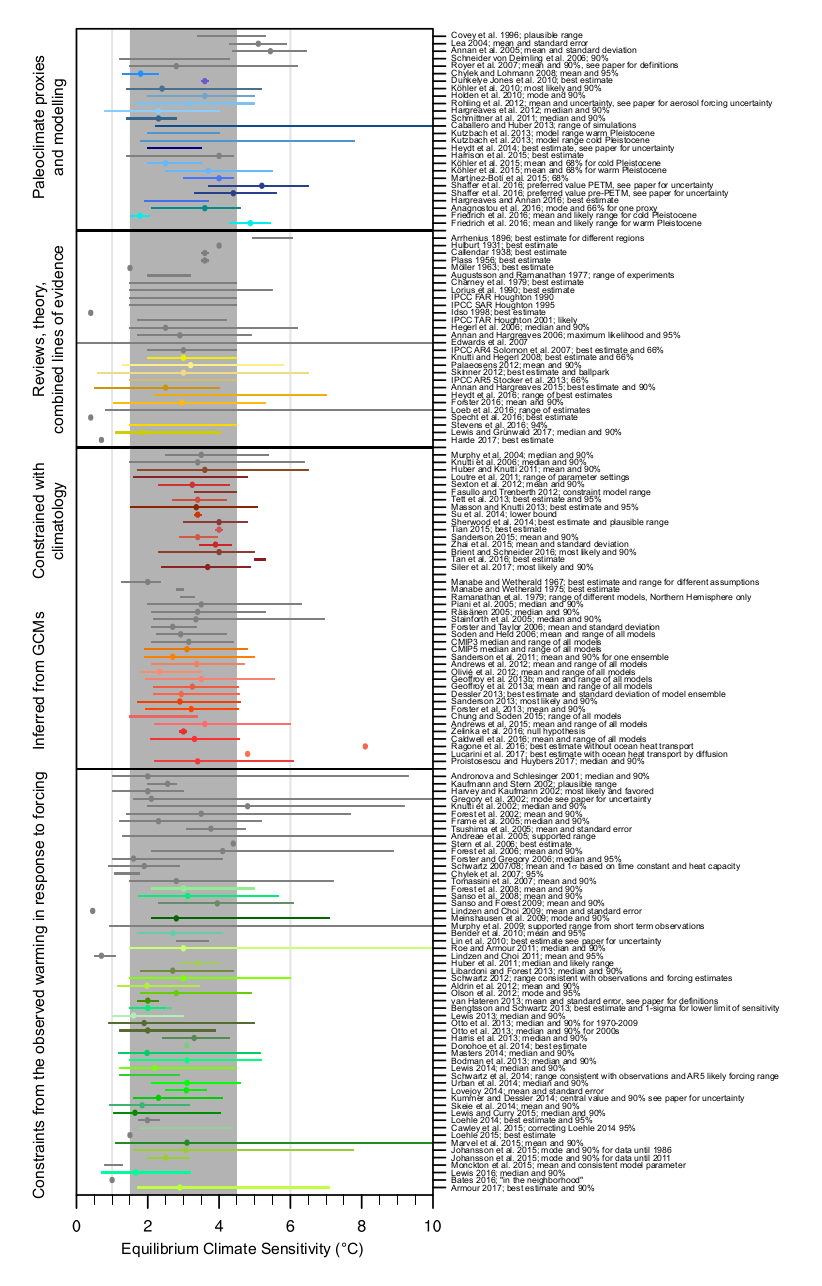
\includegraphics[width=.35\linewidth]{pic/ecs_supp_table.png}
        % \animategraphics[loop,autoplay,width=.5\linewidth]{2}{gif/volcanoe/volcanoe_}{0}{3}
        \visible<2>{
            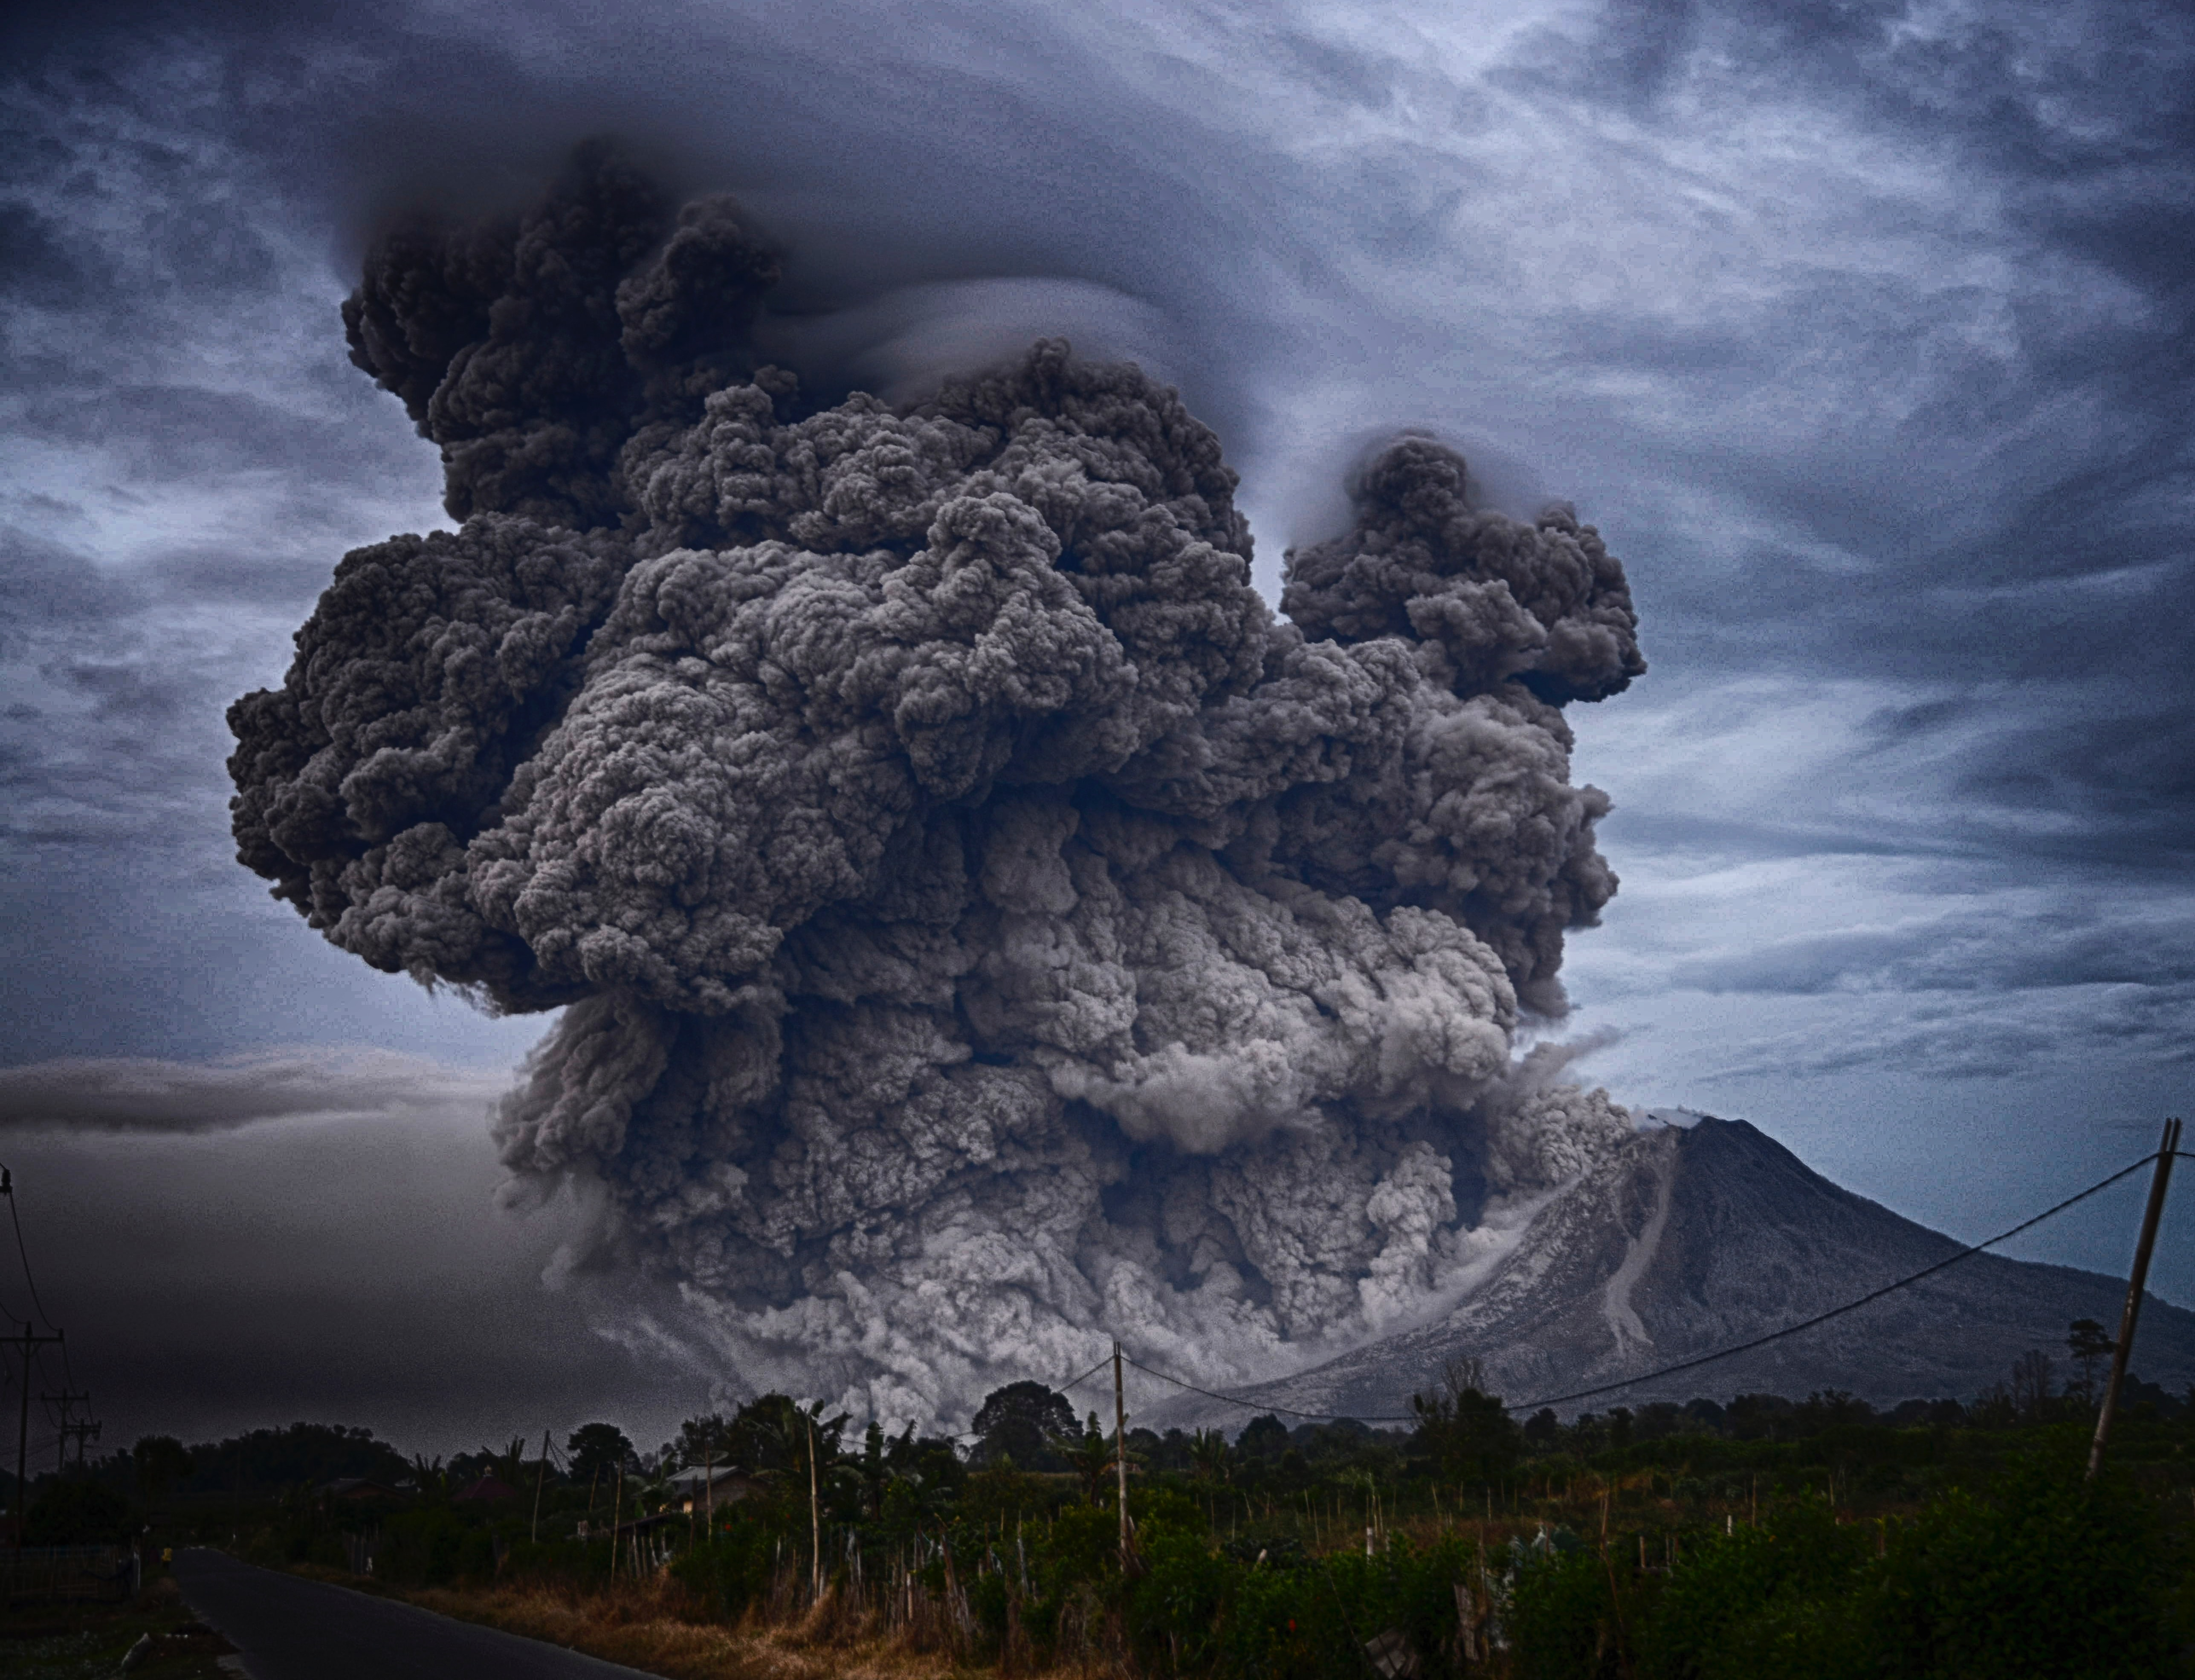
\includegraphics[width=.5\linewidth]{unsplash/volcano-unsplash.jpg}
            % 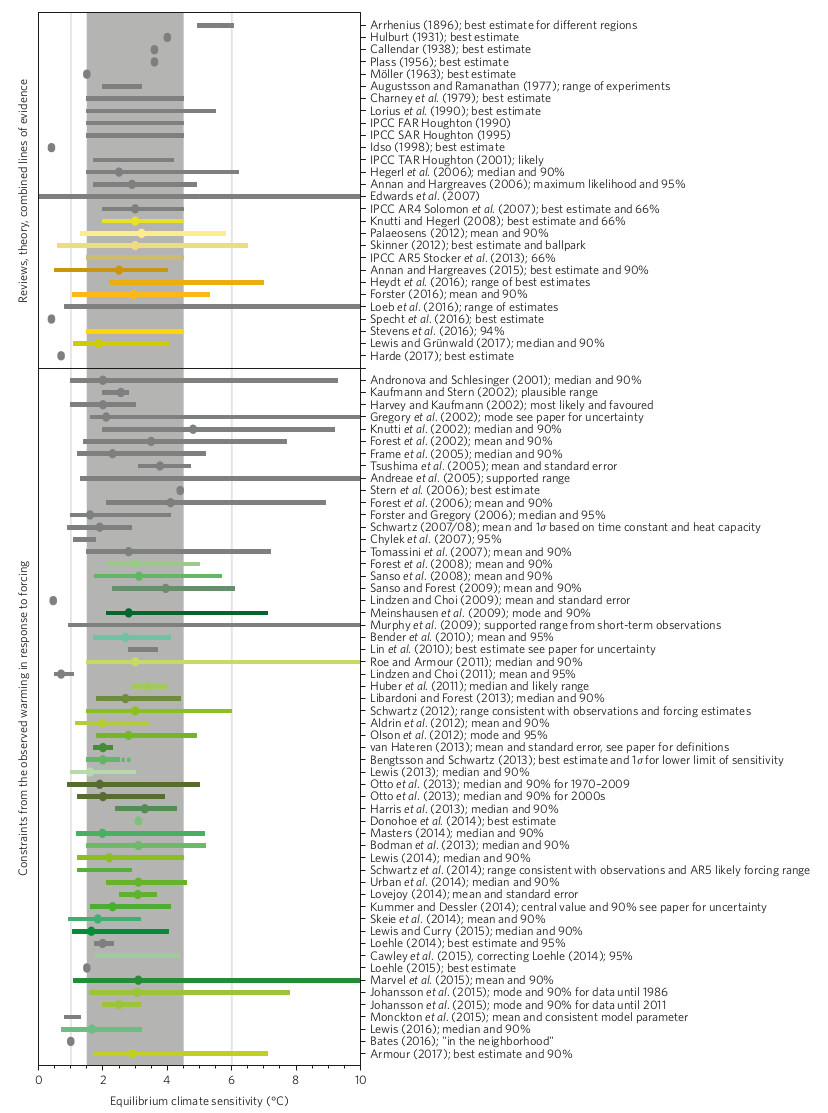
\includegraphics[width=.4\linewidth]{pic/equilibrium_climate_sensitivity.png}
        }
    \end{figure}
    \figurecite{knutti2017}

    \note<+>{
        \begin{itemize}
            \item On the right: each line is one paper/study
            \item On the left: best estimate of ECS from given study, with range in
                horisontal from 0 to 10
            \item IPCC ``likely'' region from 1.5 to 4.5
            \item Conclusion: it is difficult and literature do not agree,
                therefore, different methods are used, e.g. volcanoes
        \end{itemize}
    }
    \note<+>{
        \begin{itemize}
            \item ``Compared to anthropogenic and other natural forcings in the
                climate system, the volcanic radiative forcing acts on an short
                time scale, making the forcing and the proceeding system response
                comparatively easy to observe.''
        \end{itemize}
    }

\end{frame}

\subsection{Key points}

\begin{frame}{Key points}

    \begin{itemize}
        \item Estimate global temperature response and climate sensitivity
        \item Volcanoes produce strong temperature fluctuations
        \item Non-parametric approach
    \end{itemize}

    \note{
        \begin{itemize}
            \item Want to estimate global temperature response to volcanic
                eruptions, and possibly also climate sensitivity
            \item We know volcanoes produce strong temperature fluctuations and
                aim to infer the response from these eruptions
            \item How is this work different from other approaches? This is
                done using a non-parametric approach
        \end{itemize}
    }

\end{frame}
